\section{Visuelle detaljer}


\subsection{Ikoner}
Figur \ref{fig:appikoner} presenterer alle applikasjonsikonene som brukes til vinduene i programmet. Alle ikoner til subvinduer er satt sammen av våre egne ikoner og "<open source">-ikoner (se \ref{subssec:utvmiljo}, side \pageref{subssec:utvmiljo}). Hensikten med slike komposittikoner er at de skal gi en mer visuell tilbakemelding til brukeren som viser hvilken aktuelle funksjon som som brukes i programmet. 

\begin{figure}[ht!]
\centering
\begin{subfigure}[b]{0.2\textwidth}
\centering

\includegraphics[scale=0.4]{./img/produktdokumentasjon/visuelle_detaljer/boligLogo.png}
\caption{Programikonet}
\end{subfigure}
\quad
\begin{subfigure}[b]{0.2\textwidth}
\centering

\includegraphics[scale=0.4]{./img/produktdokumentasjon/visuelle_detaljer/ny_bolig.png}
\caption{Ny bolig}
\end{subfigure}
\quad
\begin{subfigure}[b]{0.2\textwidth}
\centering

\includegraphics[scale=0.4]{./img/produktdokumentasjon/visuelle_detaljer/ny_utleier.png}
\caption{Ny utleier}
\end{subfigure}
\quad
\begin{subfigure}[b]{0.2\textwidth}
\centering

\includegraphics[scale=0.4]{./img/produktdokumentasjon/visuelle_detaljer/edit.png}
\caption{Endre}
\end{subfigure}
\quad
\begin{subfigure}[b]{0.2\textwidth}
\centering

\includegraphics[scale=0.4]{./img/produktdokumentasjon/visuelle_detaljer/foresporsel.png}
\caption{Forespørsel}
\end{subfigure}
\quad
\begin{subfigure}[b]{0.2\textwidth}
\centering

\includegraphics[scale=0.4]{./img/produktdokumentasjon/visuelle_detaljer/bildevindu.png}
\caption{Bilder}
\end{subfigure}
\quad
\begin{subfigure}[b]{0.2\textwidth}
\centering

\includegraphics[scale=0.4]{./img/produktdokumentasjon/visuelle_detaljer/passord.png}
\caption{Pålogging}
\end{subfigure}
\quad
\caption{Applikasjons og vinduikoner}\label{fig:appikoner}
\end{figure}


\subsection{Presentasjon}
Figur \ref{fig:presentasjon} viser eksempel på hvordan objektene vises i \texttt{JEditorPane} gjennom \texttt{html}-visning. Datafelt for objektet "pareses" i klassen \texttt{ControllerOutput.java} i en metodene som er tilpasset til visning av spesifikt objekt, f.eks boligobjektene vises gjennom \texttt{visBoligObjektHTMLOutput(Object valgtObjekt, JEditorPane output, AbstraktArkfane vindu, HashSet<Bolig> boligliste)}. Det er noen begrensninger i forhold til html visningen da \texttt{JEditorPane} er kun kapabel til visning av Html versjon 3.2 og CSS 1.0 (release fra år 1997). 

\begin{figure}[ht!]
 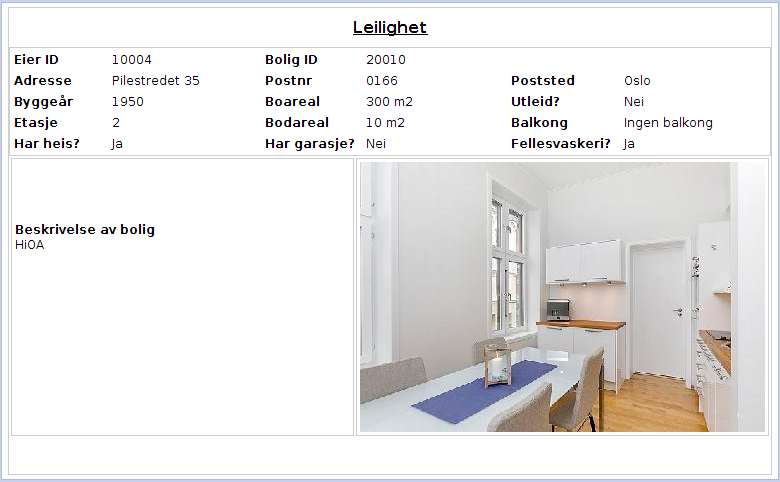
\includegraphics[width=\textwidth,height=\textheight,keepaspectratio]{./img/produktdokumentasjon/visuelle_detaljer/presentasjon.png}
 \caption{HTML presentasjon av et boligobjekt.}
 \label{fig:presentasjon}
\end{figure}


\subsection{Tabell}
I figur \ref{fig:tabell} presenteres utseende på formatert tabellobjekt, der annenhver rad har en annen bakgrunnsfarge og får en tredje bakgrunnsfarge ved markering. Forskjellige farger brukes i tillegg til horisontale linjer med hensikt å oppnå en bedre avskilt linje mellom presentasjonen av tabellkomponenter. Alle tabeller i programmet har også inkludert en meny som hører til de forskjellige objektene utfra hvilke funksjoner i programmet som kan brukes på et vist objekt. For eksempel i en tabell over boligobjekter. Boligobjekter kan man endres, slettes eller endre publiseringsstatus. Dersom brukeren "skriver ut" innhold i utleierregisteret vil det bli presentert alternativer som er spesifikke for objekter som instansierer superklassen person (ny endre, slett) men i tillegg funksjoner som er spesifikke for klassen utleier (som presentert i den refererte figuren). I eksemplet har vi mulighet å markere en person direkte og gå til registreringsdialog for bolig som da registreres på den personen. Vi kan også editere boliger som tilhører denne eieren eller også slette dem. Sammen funksjonalitet er også da tilgjengelig via den vanlige og synlige gui-komponenter som knapper eller også gjennom å dobbelklikker i tabellen.

\begin{figure}[ht!]
\center
 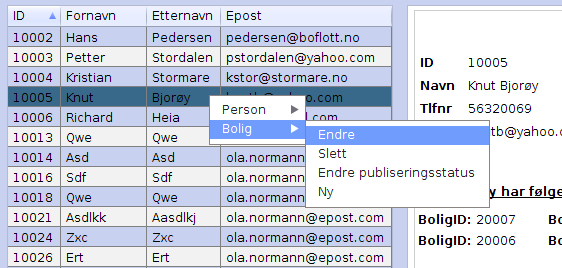
\includegraphics[scale=0.7]{./img/produktdokumentasjon/visuelle_detaljer/tabell.png}
 \caption{Visning og markering i tabell}
 \label{fig:tabell}
\end{figure}

\subsection{Grafisk tema}
Med tanke på å få bedre portabilitet mellom forskjellige operativsystem er standard Java "<LookAndFeel"> endret fra \texttt{Metal} til det nyeste swing tema \texttt{Nimbus}. Den primære årsaken til dette er at det ble observert noen forskjeller på størrelse og layout av gui-komponenter mellom operativsystemene som programmet var testet på. Eksempelvis, dersom programmet testes i Linux miljø finnes det ingen "<native"> grafisk miljø i form av komponenter som knapper, men på Mac OS der Java er kapabel å renderere standard knapper for systemet ble det noen forskjeller mellom slike komponenter\footnote{Etter tester på Mac OS og Windows.}. Bruk av nimbus som primær tema for gui komponenter gir sikkerhet at alle kompoenentene kommer til å bli renderert gjennom JVM hvilket gir en god portabilitet mellom operativsystemene (vi referer til avsnitt \ref{subsec:portabilitet}, side \pageref{subsec:portabilitet}).

\begin{figure}[ht!]
\centering
\begin{subfigure}[b]{\textwidth}
\centering
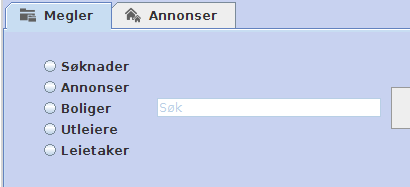
\includegraphics[scale=0.6]{./img/produktdokumentasjon/visuelle_detaljer/metal.png}
\caption{Stadard tema "<metal">}
\end{subfigure}



\begin{subfigure}[b]{\textwidth}
\centering
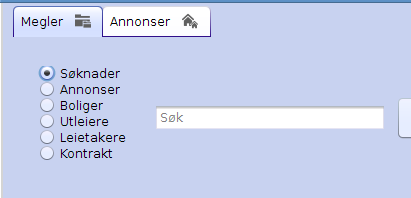
\includegraphics[scale=0.6]{./img/produktdokumentasjon/visuelle_detaljer/nimbus.png}
\caption{Nimbus}
\end{subfigure}
\caption{Applikasjons og vinduikoner}\label{fig:tema}
\end{figure}